
% This is an example file and is hereby explicitly put in the
% public domain.
%
\documentclass[ppgc,plano-doutorado, english]{iiufrgs}


% Use unicode
\usepackage[utf8]{inputenc}   % pacote para acentuação
\usepackage{booktabs}
\usepackage{caption}
\usepackage{tabularx}
\usepackage{array,color,colortbl}
\usepackage{comment}

% Necessário para incluir figuras
\usepackage{graphicx}           % pacote para importar figuras


\usepackage{times}              % pacote para usar fonte Adobe Times
% \usepackage{palatino}
% \usepackage{mathptmx}          % p/ usar fonte Adobe Times nas fórmulas

\usepackage[alf,abnt-emphasize=bf]{abntex2cite}	% pacote para usar citações abnt

%
% Informações gerais
%
\title{Improving Internet Cartography from a Different Point of View}

\author{Mazzola}{Fabrício Martins}

% orientador e co-orientador são opcionais (não diga isso pra eles :))
\advisor[Prof.~Dr.]{Barcellos}{Marinho Pilla}
%\coadvisor[Prof.~Dr.]{Claffy}{Kimberly C.}

% a data deve ser a da defesa; se nao especificada, são gerados
% mes e ano correntes
\date{October}{2018}

% o local de realização do trabalho pode ser especificado (ex. para TCs)
% com o comando \location:
%\location{Itaquaquecetuba}{SP}

% itens individuais da nominata podem ser redefinidos com os comandos
% abaixo:
% \renewcommand{\nominataReit}{Prof\textsuperscript{a}.~Wrana Maria Panizzi}
% \renewcommand{\nominataReitname}{Reitora}
% \renewcommand{\nominataPRE}{Prof.~Jos{\'e} Carlos Ferraz Hennemann}
% \renewcommand{\nominataPREname}{Pr{\'o}-Reitor de Ensino}
% \renewcommand{\nominataPRAPG}{Prof\textsuperscript{a}.~Joc{\'e}lia Grazia}
% \renewcommand{\nominataPRAPGname}{Pr{\'o}-Reitora Adjunta de P{\'o}s-Gradua{\c{c}}{\~a}o}
% \renewcommand{\nominataDir}{Prof.~Philippe Olivier Alexandre Navaux}
% \renewcommand{\nominataDirname}{Diretor do Instituto de Inform{\'a}tica}
% \renewcommand{\nominataCoord}{Prof.~Carlos Alberto Heuser}
% \renewcommand{\nominataCoordname}{Coordenador do PPGC}
% \renewcommand{\nominataBibchefe}{Beatriz Regina Bastos Haro}
% \renewcommand{\nominataBibchefename}{Bibliotec{\'a}ria-chefe do Instituto de Inform{\'a}tica}
% \renewcommand{\nominataChefeINA}{Prof.~Jos{\'e} Valdeni de Lima}
% \renewcommand{\nominataChefeINAname}{Chefe do \deptINA}
% \renewcommand{\nominataChefeINT}{Prof.~Leila Ribeiro}
% \renewcommand{\nominataChefeINTname}{Chefe do \deptINT}

\urlstyle{same}

\graphicspath{ {./images/} }

\begin{document}
    
\maketitle

\tableofcontents

\chapter{Introduction}\label{cap:introduction}
\thispagestyle{empty}

	\textbf{Context.} Peering infrastructures, such as colocation facilities and Internet Exchange Points (IXPs) are increasingly deployed all over the world, supporting a growing number of network members and peering interconnections \cite{Giotsas:2017:DPI:3098822.3098855}. Colos are physical locations that provide essential infrastructure as power, space and supports interconnection of networks. IXPs are physical infrastructures and provide a shared switching fabric where participating networks can interconnect their routers. \cite{Giotsas:2015:MPI:2716281.2836122}

	Brazil peering infrastructure maintains the largest set of public IXPs in a single country and is among the world’s top ten IXPs in terms of traffic.~\cite{DissectingBrazilianIXP}. Currently, there are 31 public IXPs deployed in all regions~\cite{IXbr}. Access to privileged data (i.e., flows samples and BGP information) of the major IXPs of the IX.br Project (e.g., IX-SP and IX-RS) leaves large room to explore measurement studies. 

	Understand if leveraging IXPs as vantage points, performing measurements campaigns from IXP to the outside Internet, and using available privileged data (i.e., flows samples and BGP information) can improve the interconnection mapping to facilities and create a broader, more accurate and scalable methodology which would be used to enhance network infrastructure and safety.


	\textbf{Motivation.} Expand existing results would provide a broader and more accurate interconnection mapping which would help to pinpoint outages and attacks, troubleshoot network problems, track traffic flows and improve the resilience of interconnections more precisely.
	%TODO colocar algumas referencias para trabalhos sobre isso

	Recent methodologies \cite{Giotsas:2015:MPI:2716281.2836122} provide accurate results but can not scale to large scenarios with several coloc, IXPs and ASes, given the large amount of active probing campaigns needed. The initial process of mapping networks, and IXPs to facilities is manual and time-consuming to be developed/updated. The work of \cite{Giotsas:2017:DPI:3098822.3098855} combines BGP communities with a colocation map to infer the location of outages. However, the map is done similarly as in \cite{Giotsas:2015:MPI:2716281.2836122}. Besides, BGP communities have no standardized semantics and are only employed by half of the BGP paths announced on the Internet.


	\textbf{Expected contributions.} We expect that leveraging IXPs as vantage points, given their global role seeing traffic from a large fraction of the Internet~\cite{Chatzis:2013:BUL:2504730.2504746}, and using available privileged data (i.e., flows samples and BGP information) will enable higher visibility and knowledge about the geolocalization of colocation facilities, and will allow creating a broader and more accurate interconnection mapping to facilities. 


	\textbf{Outline of the proposal.} Chapter~\ref{cap:background} provides background and terminology. Chapter~\ref{cap:related-work} presents the state-of-the-art and the main related work. In Chapter~\ref{cap:proposal}, we present the proposal work. Chapter~\ref{cap:expected-results} provides the expected results and main contributions. In Chapter~\ref{cap:methodology}, we show the expected methodology, set of steps and schedule. Finally, in Chapter~\ref{cap:coursework}, we present the expected coursework of the Ph.D. course.




\chapter{Peering Infrastructures}\label{cap:background}
\thispagestyle{empty}

	%In this chapter, we present some background related to the area of the proposed plan. In Section~\ref{sec:peering-infra}, we describe the concepts of Peering Infrastructures, defining Internet Exchange Points (Subsection~\ref{subsec:ixp}) and Colocation Facilities (Subsection~\ref{subsec:colos}).

	%\section{Peering Infrastructures}
	%\label{sec:peering-infra}

	Peering infrastructures are comprised of both Internet exchange points (IXP) and colocation facilities. They are responsible for exchanging a growing volume of traffic between different networks, support thousands of network members, and are widely available all over the world.

	%The studies mentioned below show that these infrastructures are worldwide available and have a comprehensive view of the Internet. Thus, they present an potential opportunity for generating rich geolocation inferences and improve knowledge about the Internet topology.

	\section{Internet Exchange Points}
	\label{subsec:ixp}

	Internet Exchange Points are physical network infrastructures where a set of autonomous systems can interconnect their networks to exchange traffic. Figure~\ref{fig:ixp-topology} shows a typical IXP architecture. IXPs provide a shared switching fabric where participating networks can interconnect their routers. The switch fabric carries the traffic resulting from public and private peering of all interconnected ASes. Each IXP provides one or more \emph{core switches} in the shared fabric for redundancy. They also associate with several Colocation Facilities and install \emph{access switches} to reach city-level interconnection with other networks~\cite{Giotsas:2015:MPI:2716281.2836122}.

	\begin{figure}[t]
	    \centering
	    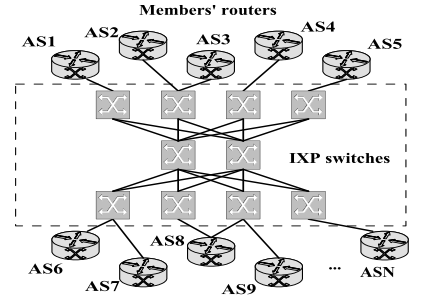
\includegraphics[width=0.5\textwidth]{ixp-topology.png}
	    \caption{A typical IXP architecture~\cite{Ager:2012}}
	    \label{fig:ixp-topology}
	\end{figure}

	Historically, IXPs can be considered as the successors of Network Access Points (NAPs), which were responsible for the smooth transition from the monolithic government network to the modern Internet~\cite{Chatzis:2013}. Since 1995, the four existing NAPs have been replaced by more than 800 IXPs in 200+ cities around the world, interconnecting 50k+ networks~\cite{Ager:2012, Giotsas:2015:MPI:2716281.2836122}.

	Studies reveal that existing Internet Exchange Points are responsible for transferring amounts of data similar to Tier 1 Internet Service Provider (ISPs)~\cite{Ager:2012}. Chatzis et al. ~\cite{Chatzis:2013:BUL:2504730.2504746} report that one of the largest European IXPs can observe traffic from a large portion of the Internet, including 42K+ routed ASes, almost all 450K+ routed prefixes and around a quarter billion IP addresses from all the countries around the globe. 

	Richter et al.~\cite{Richter:2014} point a growth of 10-20\% annually in the membership rates of ASes connecting in IXPs of 50-100\% per year in traffic rates. Kotronis et al.~\cite{Kotronis:2015:IPI:2745844.2745877} show that about 40\% of IP prefixes advertised on the Internet can be reached directly from around 5 IXPs. Besides, despite the focus to deploy peering infrastructures in Europe and USA~\cite{Chatzis:2013, Chatzis:2015:QVO:2717646.2717650}, studies reveal that developing regions as Latin America, and Africa are recently increasing the adoption of IXPs to enhance network performance~\cite{DissectingBrazilianIXP, Fanou:2017:ICC:3131365.3131394}.

	%\cite{Chatzis:2013, Chatzis:2015:QVO:2717646.2717650, IXPInternetSociety}

	\section{Colocations Facilities}
	\label{subsec:colos}

	Colocation facilities (Colos) are physical locations which provide essential infrastructures like power, space, cooling, physical security, and storage to their associated autonomous systems. More specifically, it is a place where operators of multiple networks place their networking equipment for interconnection~\cite{BITAG}. The provided amenities lower the infrastructure costs and drive small and medium providers to house their equipment (storage, server, routers) in the Colos.

	The Colos platform connects the member's network to various IXPs, transit networks, cloud/content providers and other ASes in multiple locations worldwide. In large metropolitan areas, a colocation facility operator may install various facilities in the same city, interconnected, to allow access from ASes present at one facility to networks at another facility in the same region~\cite{Giotsas:2015:MPI:2716281.2836122}. Large carrier-neutral companies such as Equinix and Telehouse are the leading operators of colocation facilities all over the world~\cite{Kotronis:2017:STC:3131365.3131388}. 

	


	

\chapter{Related Work}\label{cap:related-work}
\thispagestyle{empty}

	We now present the state-of-the-art on the main topics related to the proposed work. 
	%To elucidate the importance and evolving role of peering infrastructures in the Internet topology, in Subsection~\ref{sec:rel-work-peering-infra} we discuss the most relevant studies that analyze the operational and internal characteristics of these infrastructures. 
	%In Subsection~\ref{sec:rel-work-relat-as}, we present the efforts to identify the type of peering relationships between ASes and how this classification can increase knowledge about aspects of the networks, such as geolocation. 
	%Mapping of peering interconnections and topology elements to physical locations improve understanding of network performance and resilience. The main related work tries to improve the accuracy of this mapping and are discussed in Subsection~\ref{sec:rel-work-mapping-peer} and \ref{sec:rel-work-mapping-topo-elem}, respectively.
	In Section~\ref{sec:rel-work-mapping-peer} and Section~\ref{sec:rel-work-mapping-topo-elem}, we present the efforts to improve the accuracy of mapping peering interconnections and topology elements to physical locations, respectively. The work mentioned in these sections presents valuable and solid geolocation and infrastructure inferences. However, they either do not scale, relying on a large number of active measurements or have limited scope, providing rich inferences for just a subset of topology elements. The drawbacks reveal vast potential and opportunity to improve the generation of geolocation knowledge.

	%\section{Relationship between ASes}
	%\label{sec:rel-work-relat-as}

	%\cite{Giotsas:2014:ICR:2663716.2663743, Giotsas:2013, Luckie:2013:RCC:2504730.2504735}

	\section{Mapping of peering interconnections and infrastructures}
	\label{sec:rel-work-mapping-peer}

	Measuring and mapping the Internet at AS-level is valuable to understand the underlying structure of the topology. However, mapping at this level considerably abstracts rich information about connectivity between networks at the Internet. Accurate knowledge of interconnection geolocation helps network troubleshooting, outage detection, and attack diagnosis. Recent efforts attempt to infer peering matrices (i.e., who peers with whom at which IXP) and map interconnections to physical locations where they occur. 

	Augustin et al.~\cite{Augustin:2009:IM:1644893.1644934} proposes a method to infer peering interconnections established at IXPs, identify IXP-specific peering matrices and better understand the IXP substrate of the Internet’s AS-level ecosystem. The mechanism detected 278 IXPs and discovered the existence of about 44K IXP-related peering links. However, the method is costly both in time and number of active measurements. 

	Giotsas et al.~\cite{Giotsas:2015:MPI:2716281.2836122} propose an algorithm to infer the physical interconnection facility where an interconnection occurs among all possible candidates. The methodology provides accurate results but is unable to scale to large scenarios involving several colocation facilities, IXPs and ASes, given a large amount of active probing resources needed. The initial process of mapping networks and IXPs to facilities, required by the methodology, is manual and time-consuming to be developed/updated. Additionally, the methodology has a significant limitation because of the complexity to reproduce results and to apply it to other contexts.

	%\cite{Giotsas:2015:MPI:2716281.2836122} propose an algorithm to infer the physical interconnection facility where an interconnection occurs among all possible candidates. Uses data from PeeringDB, PCH, IXP, ASes and Network Operating Centers (NOCs) sites and lists provided in regional consortia of IXPs to build an initial mapping between AS, IXP, and facilities.
	%Measurements from RIPE Atlas, Looking Glass, iPlane and CAIDA Ark.
	
	%Methodology provides accurate results for the interfaces that resolve to a facility in a low number of iterations. Key insight is that the type of peering for an interconnection sufficiently constrains the number of candidate facilities to identify the specific facility where a given interconnection occurs.
	
	%Unable to scale to large scenarios involving several colocation facilities, IXPs, and ASes, given a large amount of active probing campaigns needed. Initial process of mapping networks and IXPs to facilities, required by the methodology, is extremely manual and time-consuming to be developed/updated. Methodology is very sensitive to missing or incorrect information and could yield inaccurate results. 

	\section{Mapping of topology elements}
	\label{sec:rel-work-mapping-topo-elem}


	Mapping network elements accurately to physical locations is a crucial task. Precise knowledge of router geolocation helps to detect BGP threats, estimate the geographic presence of ASes, and customize content delivery. It is possible to geolocate IP addresses through public or commercial databases, delay-based or DNS-based methods.

	\textbf{Geolocation databases.} Gharaibeh et al.~\cite{Gharaibeh:2017:LRG:3131365.3131380} compare router geolocation coverage and reliability in four popular geolocation databases. The authors show that despite having a  high coverage at country-level, databases are not accurate in geolocating routers at neither country- nor city-level, even if they agree significantly among each other. Poese et al.~\cite{Poese:2011:IGD:1971162.1971171} evaluates five IP geolocation databases. The results show that the vast majority of entries in the databases are biased to few popular countries. For example, a single country (e.g., United States) concentrates more than 45\% of the entries in these databases. Besides, the entries do not reflect official IP allocations and BGP routing tables.

	\textbf{Delay-based.} Topology-based Geolocation (TBG)~\cite{Katz-Bassett:2006:TIG:1177080.1177090} converts Internet route measurements from landmarks to target into constraints to geolocate the target and all of the routers along the path. The drawback is that the methodology is very sensitive to measurement errors, such as inflated latencies. GeoPing~\cite{Padmanabhan:2001:IGM:383059.383073} uses active delay measurements and needs landmarks with known geographic locations to geolocate a target host. It combines measurements to estimate the coordinates of a host. However, the geolocation of a target can only be accurately predicted if there is a landmark near the target host.

	\textbf{DNS-based.} The work of Huffaker et al.~\cite{Huffaker:2014:DDR:2656877.2656879} and Scheitle et al.~\cite{8002903} propose methods to geolocate routers based on geography-related strings in hostnames and validate the results with active measurements from different decentralized probes. Despite showing accurate results, the scope of both proposals is restricted since only a small subset of routers have apparent geographic hints in their DNS names. For example, ~\cite{Huffaker:2014:DDR:2656877.2656879} mention that only 3.6M of nearly 19M nodes ($\sim$19\%) in their dataset have apparent geographic hints in their DNS names. 

	%\cite{Gharaibeh:2017:LRG:3131365.3131380, Huffaker:2014:DDR:2656877.2656879, 8002903}

	%\cite{Gharaibeh:2017:LRG:3131365.3131380} shows that current commercial and public databases are not accurate in geolocating router at neither country- nor city-level. \cite{Huffaker:2014:DDR:2656877.2656879, 8002903} propose methods to accurately geolocate routers based on geography-related strings in hostnames and validate the results with active measurements from different decentralized probes. However, their scope is restricted since only a small subset of routers have apparent geographic hints in their DNS names.

	%The work of \cite{Giotsas:2017:DPI:3098822.3098855} combines location-tagging BGP Communities with a colocation map to infer the location of outages. Map is done similarly as in \cite{Giotsas:2015:MPI:2716281.2836122}. BGP communities have no standardized semantics and are only employed by half of the BGP paths announced on the Internet, which could lead to an incorrect and incomplete view of the infrastructure.


\chapter{Proposed Work}\label{cap:proposal}
\thispagestyle{empty}

	%Investigate if leveraging IXPs as scalable vantage points, performing measure- ments campaigns from IXP to the outside Internet, and using available privileged data (i.e., flows samples and BGP information) can improve the interconnection mapping to facilities and create a broader, more accurate and scalable methodology which would be used to enhance network infrastructure and safety. Investigate if using IXPs as vantage points could improve the initial IXP/AS to facility mapping through measurements in- stead of relying on online resources (PeeringDB, IXPs/ASes websites).

	The recent studies on the characteristics of Internet Exchange Points show the potential of these infrastructures for the emergence of new solutions involving Internet mapping. Their central roles in topology enable higher visibility and knowledge about the network, showing potential in generating geolocation inferences.

	This Ph.D. work plan seeks to investigate techniques to explore Internet Exchange Points as vantage points to improve the Internet mapping and generate geolocation inferences of peering interconnections and topology elements.  We aim to produce a hybrid approach combining the advantages of both active (i.e., accuracy) and passive (i.e., scalability) solutions. First, our method intends to perform active measurements campaigns from inside of the IXP to obtain a preliminary geolocation knowledge about the Internet topology. Next, we plan to gather already collected information on control and data planes (e.g., BGP) and correlate with the active measurement data previously obtained to increase the accuracy of the generated inferences. Finally, we will use other available public and private data sources (e.g., flow samples) to validate our results.

	Our goal is to develop a methodology that is, at the same time, \emph{accurate}, \emph{scalable} and \emph{systematic}. More specifically, it must be: ($i$) \emph{accurate} by providing valid, reliable, and correct geolocation conclusions; ($ii$) \emph{scalable} by using few but key vantage points and generating little processing and networking overhead; and ($iii$) \emph{systematic} by not relying in complex and ad-hoc solutions. We intend to produce a methodology that can be used by academia and industry for the development of new research and by network operators to apply to practical situations. We plan to deploy and validate our methodology using the Brazilian IX ecosystem, to which we have access.

	First, we aim to enhance geolocation inferences in developing regions such as Latin America, which show rich, but weakly examined, peering infrastructures~\cite{IXbr, DissectingBrazilianIXP}. Next, we aim to extend our methodology to other worldwide available IXPs and develop a better understanding of the geolocation characteristics of these infrastructures in the Internet Topology.

	%\textbf{Data to be used.} We can use data sources as PeeringDB, PCH, DataCenterMap, Inflect Data Center and Peering Mapping (https://inflect.com), IXP, ASes, and Network Operating Centers (NOCs) websites and lists provided in regional consortia of IXPs, as well as active measurements using the IXP as a vantage point to build a mapping between AS, IXP, and facilities. We can use other vantage points as RIPE Atlas, Looking Glass (Periscope \cite{Periscope}), iPlane and CAIDA Ark to augment our mapping or to validate the mapping obtained from the IXP point of view. We can use datasets of BGP to leverage the BGP Communities attribute and acquire accurate location information for about half of all BGP IPv4 updates as \cite{Giotsas:2017:DPI:3098822.3098855}. We can use flow sample datasets from IX.br to investigate how many IXPs a given flow is traversing, infer and "see" from where traffic arrives, leaves, where it comes from. Also to obtain the ground truth of this IXP’s public peering fabric, map MAC addresses to router IP addresses and their respective AS numbers~\cite{Ager:2012} and information about how two parties of an IXP peering use that link and for what purpose~\cite{Richter:2014}.

	%\textbf{Assumptions.}

	%\textbf{Set of metrics.} Number of peering interfaces inferred. Fraction of resolved interfaces when dealing with less vantage points used. Fraction of unresolved interfaces with when removing facilities information. Fraction of ground truth locations that match inferred locations. \cite{Giotsas:2015:MPI:2716281.2836122}. Number of peering interfaces inferred by one IXP. Error probability of inferred location.

	\textbf{Research Questions.} In this work, we aim to answer the following research questions: can IXPs be used as vantage points to generate geolocation inferences about peering interconnections and Internet topology? How can we obtain accurate geolocation of infrastructure elements from inside the IXP? Is it possible to correlate active measurement data with collected information on control and data planes (e.g., BGP) to improve the Internet cartography?  Which and how many IXPs are necessary to have a precise vision of the Internet? What are the implications of using this approach concerning computational cost, network traffic, and privacy? How is it possible to measure in a scalable and automatized way?

	\textbf{Risks and limitations.} There are a few challenges and risks in the proposed research. Due to the low representation of existing measurement projects in developing areas (e.g., Latin America), there could be gaps in infrastructure and methodologies which could affect our geolocation inferences. We could face performance problems as IXPs not being good vantage points (VP) to improve Internet mapping or providing inaccurate results when using few IXPs given that their visibility, individually, may not perfect. Besides that, we could also face bureaucratic challenges as IXPs could not see a clear advantage of being used as VPs.


\chapter{Methodology}\label{cap:methodology}
\thispagestyle{empty}

\section{Set of Steps}
\label{sec:steps}

Methodology to be used.

\begin{enumerate}
\item {\bf Evaluation of state-of-the-art}: In-depth state-of-the-art study about Colocation Facilities, Internet Exchange Points, and the existing methodologies to map peering interconnections. Identify characteristics and limitations of each related work and understand better how IXPs can be leveraged as vantage points to improve interconnection mapping to facilities;

\item {\bf Preliminary modeling}: in this step, we will model a methodology capable of using IXPs as vantage points and improve interconnection mapping to facilities;

\item {\bf Preliminary evaluation}: preliminary evaluation of the previously proposed methodology, using small-scale measurements campaigns and a subset of the available data to obtain validation.;

\item {\bf Prototype development}: in this step, a prototype of the proposed methodology will be developed to perform the experimental evaluation. The objective will be to create a scalable product to be used in IXPs environments;;

\item {\bf Experimental Evaluation}: final step of the study, including large-scale evaluation, composed of campaigns of measurements and data collection, to evaluate and validate the effectiveness of the developed methodology.

\end{enumerate}

\section{Schedule}
\label{sec:schedule}

Set of steps and the schedule proposed.

\begin{enumerate}

\item In-depth state-of-the-art study about Colocation Facilities, Internet Exchange Points, and the existing methodologies to map peering interconnections; \label{it:estado-da-arte}

\item Modeling of a methodology capable of using IXPs as vantage points and improve interconnection mapping to facilities; \label{it:modelagem}

\item Qualification Exam; \label{it:qualif}

\item Examination of proficiency in a foreign language; \label{it:idioma}

\item Preliminary evaluation of the previously proposed methodology, using small-scale measurements campaigns and a subset of the available data to obtain validation and identify main attributes and limitations; \label{it:aval-anali}

\item Review and reassessment of the model in order to improve the initial modeling based on the results obtained in the performed evaluations; \label{it:rev-modelo}

\item Period reserved for doctorate sandwich; \label{it:sanduba}

\item Definition and design of the experimental evaluation; \label{it:proj-amb-exp}

\item Experimental evaluation of the proposed methodology; \label{it:aval-larga-escala}

\item Thesis Proposal Defense; \label{it:def-prop-tese}

\item Improvement of the methodology considering the results obtained in previous activities, also considering contributions and recommendations of the evaluation committee of the thesis proposal; \label{it:rev-final-modelo}

\item Thesis writing; \label{it:redacao}

\item Thesis defense; \label{it:def-tese}

\item Participation in congresses, symposia, and schools related to the theme of the thesis; \label{it:part-cong}

\item Writing and submitting articles for conferences and periodicals based on the results obtained during the studies and evaluations carried out, related to the theme of this doctoral proposal. \label{it:submissoes}
\end{enumerate}

\begin{table}[htp]
\centering
\begin{center}
% use packages: array,color,colortbl
\newcommand{\mc}[3]{\multicolumn{#1}{#2}{#3}}
\definecolor{tcA}{gray}{0.875}
\definecolor{tcB}{gray}{0.75}
\definecolor{tcC}{gray}{0.957}
%
\begin{tabular}{|>{\columncolor{tcA}}l|l|l|l|l|l|l|l|l|}\hline
% ----------- cabeçalho
\rowcolor{tcB}
\mc{1}{|>{\columncolor{tcB}}l|}{Activities} &
\mc{1}{|>{\columncolor{tcB}}l|}{2019/1} &
\mc{1}{|>{\columncolor{tcB}}l|}{2019/2} &
\mc{1}{|>{\columncolor{tcB}}l|}{2020/1} &
\mc{1}{|>{\columncolor{tcB}}l|}{2020/2} &
\mc{1}{|>{\columncolor{tcB}}l|}{2021/1} &
\mc{1}{|>{\columncolor{tcB}}l|}{2021/2} &
\mc{1}{|>{\columncolor{tcB}}l|}{2022/1} &
\mc{1}{|>{\columncolor{tcB}}l|}{2022/2} \\
\hline
% -------- Avaliação do estado-da-arte
\mc{1}{|>{\columncolor{tcA}}c|}{\ref{it:estado-da-arte}} &
\mc{1}{|>{\columncolor[gray]{0.3}}l|}{} &
\mc{1}{|>{\columncolor[gray]{0.3}}l|}{} &
\mc{1}{|>{\columncolor{tcC}}l|}{ } &
\mc{1}{|>{\columncolor{tcC}}l|}{ } &
\mc{1}{|>{\columncolor{tcC}}l|}{ } &
\mc{1}{|>{\columncolor{tcC}}l|}{ } &
\mc{1}{|>{\columncolor{tcC}}l|}{ } &
\mc{1}{|>{\columncolor{tcC}}l|}{ } \\
\hline
% -------- Modelagem inicial
\mc{1}{|>{\columncolor{tcA}}c|}{\ref{it:modelagem}} &
\mc{1}{|>{\columncolor[gray]{0.3}}l|}{} &
\mc{1}{|>{\columncolor[gray]{0.3}}l|}{} &
\mc{1}{|>{\columncolor[gray]{0.3}}l|}{} &
\mc{1}{|>{\columncolor{tcC}}l|}{ } &
\mc{1}{|>{\columncolor{tcC}}l|}{ } &
\mc{1}{|>{\columncolor{tcC}}l|}{ } &
\mc{1}{|>{\columncolor{tcC}}l|}{ } &
\mc{1}{|>{\columncolor{tcC}}l|}{ } \\
\hline
% -------- Exame de Qualificação
%\rowcolor{tcC}
\mc{1}{|>{\columncolor{tcA}}c|}{\ref{it:qualif}} &
\mc{1}{|>{\columncolor{tcC}}l|}{ } &
\mc{1}{|>{\columncolor[gray]{0.3}}l|}{} &
\mc{1}{|>{\columncolor{tcC}}l|}{ } &
\mc{1}{|>{\columncolor{tcC}}l|}{ } &
\mc{1}{|>{\columncolor{tcC}}l|}{ } &
\mc{1}{|>{\columncolor{tcC}}l|}{ } &
\mc{1}{|>{\columncolor{tcC}}l|}{ } &
\mc{1}{|>{\columncolor{tcC}}l|}{ } \\
\hline
% -------- Exame de Proficiência em Língua Estrangeira
%\rowcolor{tcC}
\mc{1}{|>{\columncolor{tcA}}c|}{\ref{it:idioma}} &
\mc{1}{|>{\columncolor{tcC}}l|}{ } &
\mc{1}{|>{\columncolor[gray]{0.3}}l|}{} &
\mc{1}{|>{\columncolor{tcC}}l|}{ } &
\mc{1}{|>{\columncolor{tcC}}l|}{ } &
\mc{1}{|>{\columncolor{tcC}}l|}{ } &
\mc{1}{|>{\columncolor{tcC}}l|}{ } &
\mc{1}{|>{\columncolor{tcC}}l|}{ } &
\mc{1}{|>{\columncolor{tcC}}l|}{ } \\
\hline
% -------- Avaliação por métodos analíticos
%\rowcolor{tcC}
\mc{1}{|>{\columncolor{tcA}}c|}{\ref{it:aval-anali}} &
\mc{1}{|>{\columncolor{tcC}}l|}{ } &
\mc{1}{|>{\columncolor{tcC}}l|}{ } &
\mc{1}{|>{\columncolor[gray]{0.3}}l|}{} &
\mc{1}{|>{\columncolor[gray]{0.3}}l|}{} &
\mc{1}{|>{\columncolor{tcC}}l|}{ } &
\mc{1}{|>{\columncolor{tcC}}l|}{ } &
\mc{1}{|>{\columncolor{tcC}}l|}{ } &
\mc{1}{|>{\columncolor{tcC}}l|}{ } \\
\hline

% -------- Revisão do Modelo
\mc{1}{|>{\columncolor{tcA}}c|}{\ref{it:rev-modelo}} &
\mc{1}{|>{\columncolor{tcC}}l|}{ } &
\mc{1}{|>{\columncolor{tcC}}l|}{ } &
\mc{1}{|>{\columncolor{tcC}}l|}{ } &
\mc{1}{|>{\columncolor[gray]{0.3}}l|}{} &
\mc{1}{|>{\columncolor{tcC}}l|}{ } &
\mc{1}{|>{\columncolor{tcC}}l|}{ } &
\mc{1}{|>{\columncolor{tcC}}l|}{ } &
\mc{1}{|>{\columncolor{tcC}}l|}{ } \\
\hline
% -------- Afastamento para doutorado sanduíche
%\rowcolor{tcC}
\mc{1}{|>{\columncolor{tcA}}c|}{\ref{it:sanduba}} &
\mc{1}{|>{\columncolor{tcC}}l|}{ } &
\mc{1}{|>{\columncolor{tcC}}l|}{ } &
\mc{1}{|>{\columncolor[gray]{0.3}}l|}{} &
\mc{1}{|>{\columncolor[gray]{0.3}}l|}{} &
\mc{1}{|>{\columncolor{tcC}}l|}{ } &
\mc{1}{|>{\columncolor{tcC}}l|}{ } &
\mc{1}{|>{\columncolor{tcC}}l|}{ } &
\mc{1}{|>{\columncolor{tcC}}l|}{ } \\
\hline
% -------- Projeto de um ambiente de experimentação
%\rowcolor{tcC}
\mc{1}{|>{\columncolor{tcA}}c|}{\ref{it:proj-amb-exp}} &
\mc{1}{|>{\columncolor{tcC}}l|}{ } &
\mc{1}{|>{\columncolor{tcC}}l|}{ } &
\mc{1}{|>{\columncolor{tcC}}l|}{ } &
\mc{1}{|>{\columncolor[gray]{0.3}}l|}{} &
\mc{1}{|>{\columncolor[gray]{0.3}}l|}{} &
\mc{1}{|>{\columncolor{tcC}}l|}{ } &
\mc{1}{|>{\columncolor{tcC}}l|}{ } &
\mc{1}{|>{\columncolor{tcC}}l|}{ } \\
\hline
% -------- Avaliação experimental em larga escala
%\rowcolor{tcC}
\mc{1}{|>{\columncolor{tcA}}c|}{\ref{it:aval-larga-escala}} &
\mc{1}{|>{\columncolor{tcC}}l|}{ } &
\mc{1}{|>{\columncolor{tcC}}l|}{ } &
\mc{1}{|>{\columncolor{tcC}}l|}{ } &
\mc{1}{|>{\columncolor{tcC}}l|}{ } &
\mc{1}{|>{\columncolor[gray]{0.3}}l|}{} &
\mc{1}{|>{\columncolor[gray]{0.3}}l|}{} &
\mc{1}{|>{\columncolor{tcC}}l|}{ } &
\mc{1}{|>{\columncolor{tcC}}l|}{ } \\
\hline
% -------- Defesa da Proposta Tese
%\rowcolor{tcC}
\mc{1}{|>{\columncolor{tcA}}c|}{\ref{it:def-prop-tese}} &
\mc{1}{|>{\columncolor{tcC}}l|}{ } &
\mc{1}{|>{\columncolor{tcC}}l|}{ } &
\mc{1}{|>{\columncolor{tcC}}l|}{ } &
\mc{1}{|>{\columncolor{tcC}}l|}{ } &
\mc{1}{|>{\columncolor{tcC}}l|}{ } &
\mc{1}{|>{\columncolor[gray]{0.3}}l|}{} &
\mc{1}{|>{\columncolor{tcC}}l|}{ } &
\mc{1}{|>{\columncolor{tcC}}l|}{ } \\
\hline
% -------- Aperfeiçoamento do modelo
\mc{1}{|>{\columncolor{tcA}}c|}{\ref{it:rev-final-modelo}} &
\mc{1}{|>{\columncolor{tcC}}l|}{ } &
\mc{1}{|>{\columncolor{tcC}}l|}{ } &
\mc{1}{|>{\columncolor{tcC}}l|}{ } &
\mc{1}{|>{\columncolor{tcC}}l|}{ } &
\mc{1}{|>{\columncolor{tcC}}l|}{ } &
\mc{1}{|>{\columncolor[gray]{0.3}}l|}{} &
\mc{1}{|>{\columncolor[gray]{0.3}}l|}{} &
\mc{1}{|>{\columncolor{tcC}}l|}{ } \\
\hline
%\rowcolor{tcC}
% -------- Redação Tese
%\rowcolor{tcC}
\mc{1}{|>{\columncolor{tcA}}c|}{\ref{it:redacao}} &
\mc{1}{|>{\columncolor{tcC}}l|}{ } &
\mc{1}{|>{\columncolor{tcC}}l|}{ } &
\mc{1}{|>{\columncolor{tcC}}l|}{ } &
\mc{1}{|>{\columncolor[gray]{0.3}}l|}{} &
\mc{1}{|>{\columncolor[gray]{0.3}}l|}{} &
\mc{1}{|>{\columncolor[gray]{0.3}}l|}{} &
\mc{1}{|>{\columncolor[gray]{0.3}}l|}{} &
\mc{1}{|>{\columncolor{tcC}}l|}{ } \\
\hline
% -------- Defesa Tese
\mc{1}{|>{\columncolor{tcA}}c|}{\ref{it:def-tese}} &
\mc{1}{|>{\columncolor{tcC}}l|}{ } &
\mc{1}{|>{\columncolor{tcC}}l|}{ } &
\mc{1}{|>{\columncolor{tcC}}l|}{ } &
\mc{1}{|>{\columncolor{tcC}}l|}{ } &
\mc{1}{|>{\columncolor{tcC}}l|}{ } &
\mc{1}{|>{\columncolor{tcC}}l|}{ } &
\mc{1}{|>{\columncolor{tcC}}l|}{ } &
\mc{1}{|>{\columncolor[gray]{0.3}}l|}{} \\
\hline
 % -------- Participação Congressos
%\rowcolor{tcC}
\mc{1}{|>{\columncolor{tcA}}c|}{\ref{it:part-cong}} &
\mc{1}{|>{\columncolor[gray]{0.3}}l|}{} &
\mc{1}{|>{\columncolor[gray]{0.3}}l|}{} &
\mc{1}{|>{\columncolor[gray]{0.3}}l|}{} &
\mc{1}{|>{\columncolor[gray]{0.3}}l|}{} &
\mc{1}{|>{\columncolor[gray]{0.3}}l|}{} &
\mc{1}{|>{\columncolor[gray]{0.3}}l|}{} &
\mc{1}{|>{\columncolor[gray]{0.3}}l|}{} &
\mc{1}{|>{\columncolor[gray]{0.3}}l|}{} \\
\hline
% -------- Redação Submissão Artigos
\mc{1}{|>{\columncolor{tcA}}c|}{\ref{it:submissoes}} &
\mc{1}{|>{\columncolor[gray]{0.3}}l|}{} &
\mc{1}{|>{\columncolor[gray]{0.3}}l|}{} &
\mc{1}{|>{\columncolor[gray]{0.3}}l|}{} &
\mc{1}{|>{\columncolor[gray]{0.3}}l|}{} &
\mc{1}{|>{\columncolor[gray]{0.3}}l|}{} &
\mc{1}{|>{\columncolor[gray]{0.3}}l|}{} &
\mc{1}{|>{\columncolor[gray]{0.3}}l|}{} &
\mc{1}{|>{\columncolor[gray]{0.3}}l|}{} \\
\hline
\end{tabular}
\end{center}
\caption{Schedule of activities during the doctoral period}
\label{tab:planejamento-doutorado}
\end{table}

\section{Collaboration}
\label{sec:collaboration}

joint work with UCSD. expands existing relationship. Second year of PhD expected to be located at CAIDA/UCSD. Funding to be determined.



\chapter{Expected Results}\label{cap:expected-results}
\thispagestyle{empty}

	In this chapter, we present the expected results of the Ph.D. First, we describe the main contributions of the proposed work in Section~\ref{sec:contributions}. Finally, in Section~\ref{sec:publications}, we present some of the leading journals (Table~\ref{tbl:journals}) in which the results obtained during the doctorate can be published and some of the main conferences related to the research areas involved in this plan (Table~\ref{tbl:conferences}).

	\section{Main Contributions of the Thesis}\label{sec:contributions}
	\thispagestyle{empty}

	The following contributions are expected with the development of the proposed work:

	\begin{enumerate}
    \item Analysis of the potential of Internet Exchange Points to be used as scalable vantage points to map and generate geolocation inferences, as well as its strengths and limitations;

    \item Formalization of a methodology to improve the mapping of peering interconnections by exploiting the characteristics of the Internet Exchange Points, introducing new datasets and scalability;

    \item Development of a prototype of the proposed methodology, allowing its applicability in practical situations and the development of new researches.
    \end{enumerate}

	It is also expected that during the development of this work there will be the participation of master and scientific initiation students, performing work related to the doctoral thesis proposed in this plan. The participation in the training of these student's knowledge is then considered as one of the possible contributions.

	\section{Publications}
	\label{sec:publications}

	The development of Ph.D. activities will generate results which will be used as a basis for the writing of articles for journals and congresses. Table~\ref{tbl:journals} presents some of the main journals in which the results obtained during the doctorate can be published, while Table~\ref{tbl:conferences} presents some of the leading conferences of the research areas involved in this plan.

	\newpage

	\begin{table}[htp]
	\centering
	\begin{tabularx}{\textwidth}{l | c | c}
	\hline
	{\bf Journal}                                           & {\bf Impact Factor} & \textbf{Qualis} \\ \hline
    \textit{Communications of the ACM}                        &      4.027        & A1 \\ \hline
	\textit{IEEE/ACM Transactions on Networking}              &      3.376        & A1 \\ \hline
	\textit{Elsevier Computer Networks}                       &      2.516        & A1 \\ \hline
	\textit{ACM CCR}                					      &      2.008        & B1 \\ \hline
	

	\end{tabularx}
	\caption{Journals related to Ph.D.}
	\label{tbl:journals}
	\end{table}

	\begin{table}[htp]
	\centering
	\begin{tabularx}{\textwidth}{ l | c | c | c }
	\hline
	{\bf Conference} & {\bf Acceptance Rate} & \textbf{H-index} & \textbf{Qualis}      \\ 
	                          							  &  &  & \textbf{2016}        \\ \hline
	\textit{ACM Internet Measurements}                    &  24.7\% & 75 & A1          \\ 
	\textit{(IMC) Conference}   						  &         &    &             \\ \hline
	\textit{Network Traffic Measurement}                  &  39.2\% & -- & --          \\
	\textit{ and Analysis Conference (TMA)}               &         &    &             \\ \hline
	\textit{Passive and Active Network}                   &  40.8\% & -- & A2          \\
	\textit{ Measurement Conference (PAM)}                &         &    &             \\ \hline
	\textit{ACM Special Interest Group on Data}           &  18\%   & 67 & A1          \\
	\textit{Communication (SIGCOMM) Conference}           &         &    &             \\ \hline
	\textit{ACM International Conference on}              &  17.2\% &    & A1          \\
	\textit{emerging Networking EXperiments}	          &         & 35 &             \\
	\textit{and Technologies(CoNEXT)}                     &         &    &             \\ \hline
	\textit{IEEE Conference on Computer}                  &  20.9\% & 80 & A1          \\
	\textit{Communications (INFOCOM)}                     &         &    &             \\ \hline
	\textit{USENIX Symposium on Networked}                &  15.4\% &    & A1          \\
	\textit{Systems Design and Implementation}            &         & 62 &             \\
	\textit{(NSDI)}             				          &         &    &             \\ \hline

	\hline
	\end{tabularx}
	\caption{Conferences related to Ph.D.}
	\label{tbl:conferences}
	\end{table}

\chapter{Coursework}\label{cap:coursework}
\thispagestyle{empty}

This chapter presents the expected coursework to be taken in PhD course. Table~\ref{tab:phd-courses} shows the courses and the number of credits that will be taken during the PhD. All courses sums a total of 20 credits, agreeing with the minimum required for the PhD.

\begin{table}[htp]
\centering
\begin{tabularx}{\textwidth}{ l | c | c | c}
\hline
{\bf Code} & {\bf Period} & \textbf{Period} & \textbf{Credits} \\ 
CMP410 & Teaching Practice I & 2019/1 & 1 \\
CMP230 & Computer System Security & 2019/1 & 4 \\
CMP182 & Computer Network & 2019/1 & 4 \\
CMP411 & Teaching Practice II & 2019/2 & 1 \\
CMP267 & Novel Internet Architectures and Paradigms & 2019/2 & 4 \\
CMP223 & Computer System Performance Analysis & 2019/2 & 4 \\
CMP600 & Qualification Exam & 2019/2 & 2 \\

\hline
\end{tabularx}
\caption{Courses to be taken in PhD}
\label{tab:phd-courses}
\end{table}



\bibliographystyle{abntex2-alf}
\bibliography{ref}

\end{document}
